\chapter{Implementation of uROS}
\section{RCLC}
This repository provides the \textit{rclc} package, which complements the ROS Client Support Library (\textit{rcl}) to make up a complete ROS 2 client library for the C programming language. That is, \textit{rclc} does not add a new layer of types on top of \textit{rcl} (like rclcpp and rclpy do) but only provides convenience functions that ease the programming with the \textit{rcl} types. New types are introduced only for concepts that are missing in \textit{rcl}, most important an Executor and a Lifecycle Node.

The API of the RCLC-Executor can be divided in several phases: \textbf{Configuration}, \textbf{Running} and \textbf{Clean-Up}.

\subsection{Configuration Phase}
During the configuration phase, the user shall define: the total number of callbacks, trigger condition (optional, default: ANY), data communication semantics (optional, default RCLCPP) and the processing sequence of the callbacks.
\subsubsection{\api{rclc\_executor\_t * rclc\_get\_zero\_initialized\_executor()}}
Returns a zero initialized executor object.

\subsubsection{\api{rclc\_executor\_init(rclc\_executor\_t * executor, rcl\_context\_t * context, const size\_t number\_of\_handles, const rcl\_allocator\_t * allocator)}}
As the Executor is intended for embedded controllers, dynamic memory management is crucial. Therefore at initialization of the RCLC-Executor, the user defines the total number of handles \textit{number\_of\_handles}. \textbf{A handle is a term for subscriptions, timers, services, clients and guard conditions.} The necessary dynamic memory will be allocated only in this phase and no more memory in the running phase. The corresponding wait-set is allocated in the first execution of the spin-method or in the optional call to \textit{rclc\_executor\_prepare}. This makes this Executor static in the sense, that during runtime no heap allocations occur. You can add, however, at runtime as many handles, e.g. subscriptions, to the executor until the maximum number of handles is reached. The \textit{context} is the RCL context, and \textit{allocator} points to a memory allocator.
\begin{figure}[htb!]
    \centering
    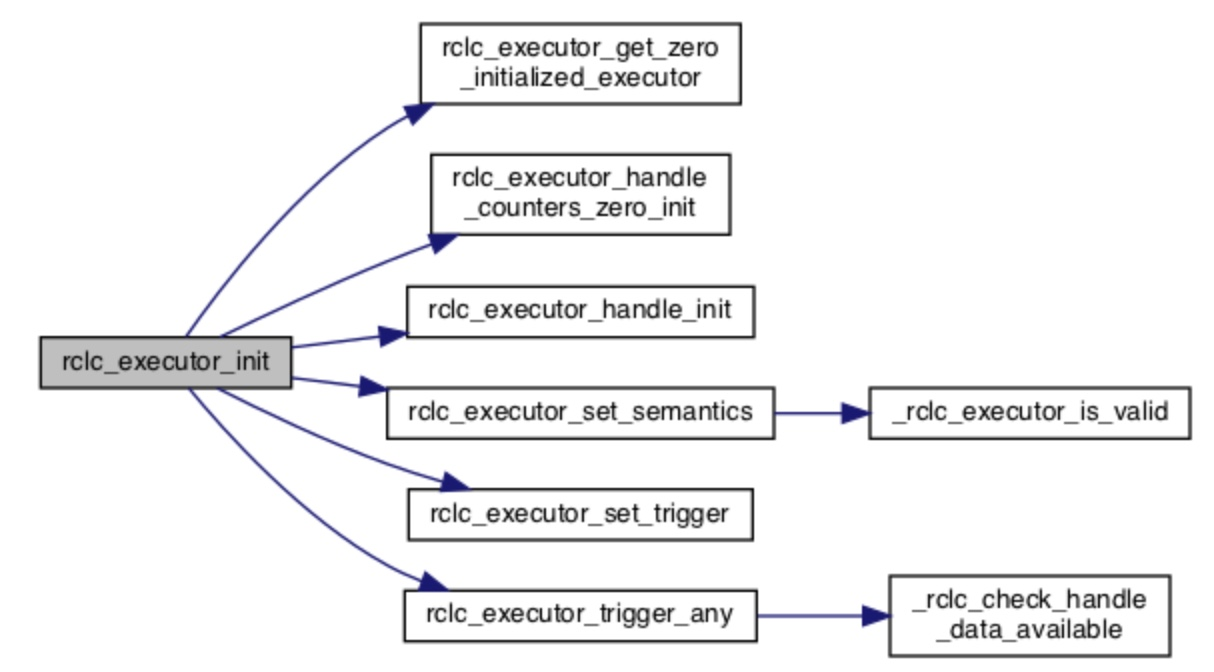
\includegraphics[width=0.95\linewidth]{Img/graph/rclc/executor_init.jpg}
    \caption{executor\_init call}
    \vspace{-0.1in}
\end{figure}

\begin{figure}[htb!]
    \centering
    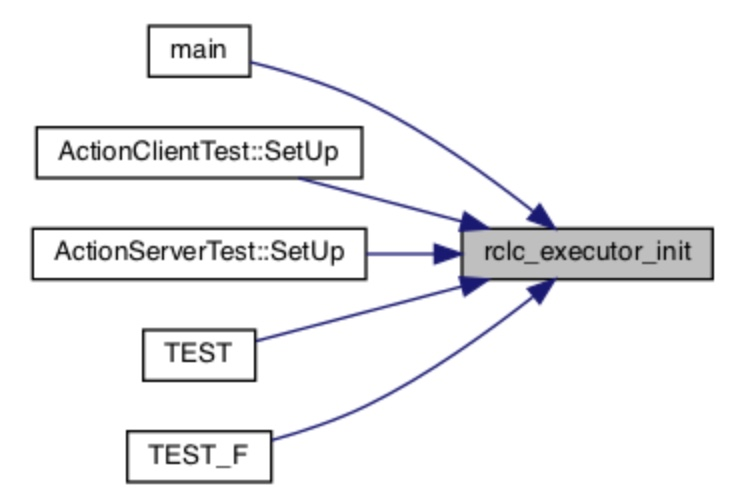
\includegraphics[width=0.75\linewidth]{Img/graph/rclc/executor_init_caller.jpg}
    \caption{executor\_init caller}
    \vspace{-0.1in}
\end{figure}


\subsubsection{\api{rclc\_executor\_set\_timeout(rclc\_executor\_t * executor, const uint64\_t timeout\_ns)}}
The timeout in nano-seconds \textit{timeout\_ns} for waiting for new data from the DDS-queue is specified in \api{rclc\_executor\_set\_timeout()} (this is the timeout parameter for \api{rcl\_wait()}).

\subsubsection{\api{rclc\_executor\_set\_semantics(rclc\_executor\_t * executor, rclc\_executor\_semantics\_t semantics)}}
The \textbf{data communication semantics} can either be \textit{RCLCPP}(default) or \textit{LET}.

To be compatible with ROS 2 rclcpp Executor, the existing rclcpp semantics is implemented with the option \textit{RCLCPP}. That is, with the spin-function the DDS-queue is constantly monitored for new data (\api{rcl\_wait()}). If new data becomes available, then it is fetched from DDS (\api{rcl\_take()}) immediately before the callback is executed. All callbacks are processed in the user-defined order, this is the only difference to the rclcpp Executor, in which the order can not be defined by the user.

The LET semantics is implemented such that at the beginning of processing, all available data is fetched (\api{rcl\_take()}) and buffered and then the callbacks are processed in the pre-defined operating on the buffered copy.

\subsubsection{\api{rclc\_executor\_set\_trigger(rclc\_executor\_t * executor, rclc\_executor\_trigger\_t trigger\_function, void * trigger\_object)}}
The trigger condition \api{rclc\_executor\_set\_trigger} defines when the processing of the callbacks shall start. For convenience some trigger conditions have been defined:
\begin{itemize}
    \item \textit{rclc\_executor\_trigger\_any(default)}: start executing if any callback has new data
    \item \textit{rclc\_executor\_trigger\_all}: start executing if all callbacks have new data
    \item \textit{rclc\_executor\_trigger\_one(\&data)}: start executing if \textit{data} has been received
    \item \textit{rclc\_executor\_trigger\_always}: returns always true, that is every time the Executor spins, the processing of the callbacks is invocated. For example with \textit{spin\_period} and this trigger condition as well as specifying all callbacks of subscriptions being called as \textit{ALWAYS}, a fixed period execution of all callbacks can be implemented, irrespective whether new data is available or not.
    \item \textit{user\_defined\_function}: the user can also define its own function with more complex logic
\end{itemize}

With the \textit{rclc\_executor\_trigger\_one} trigger, the handle to trigger is specified with \textit{trigger\_object}. In the other cases of the trigger conditions this parameter shall be \textit{NULL}.

\subsubsection{\api{rclc\_executor\_add\_subscription(rclc\_executor\_t * executor, rcl\_subscription\_t * subscription, void * msg, rclc\_subscription\_callback\_t callback, rclc\_executor\_handle\_invocation\_t invocation)} AND \api{rclc\_executor\_add\_timer( rclc\_executor\_t * executor, rcl\_timer\_t * timer)}}
To add handles to the Executor, the functions \api{rclc\_executor\_add\_subscription()} for subscriptions and \api{rclc\_executor\_add\_timer()} for timers. The order in which these functions are called, defines later the sequential processing order during runtime.

For adding a subscription, the rcl subscription handle \textit{subscription}, a pointer an allocated message \textit{msg}, the message callback \textit{callback} and an invocation option \textit{invocation} need to be specified. \textbf{The invocation option specifies}, whether the callback shall be executed only if new data is available (\textit{ON\_NEW\_DATA}) or if the callback shall always be executed (\textit{ALWAYS}). The second option is useful for example when the callback is expected to be called at a fixed rate.

For a timer, only the rcl timer object \textit{timer} is needed.

\subsubsection{\api{rclc\_executor\_prepare(rclc\_executor\_t * executor)}}
The function \api{rclc\_executor\_prepare} prepares the internal RCL wait set allocating the required dynamic memory. Its use is optional becouse it also will be checked in the spin functions. If used and no entities are added to the executor during running phase, no dynamic allocations are guaranteed during the running phase.

\subsection{Running Phase}
\subsubsection{\apiarg{rclc\_executor\_spin\_some}{rclc\_executor\_t * executor, const uint64\_t timeout\_ns}}
The function \api{rclc\_executor\_spin\_some} checks for new data from the DDS queue once. \textbf{It first copies all data into local data structures and then executes all handles according the specified order.} This implements the LET semantics. Note that memory is dynamically allocated within rcl-layer, when DDS queue is accessed with \api{rcl\_wait\_set\_init()}.

The static-LET executor performs the following actions:
\begin{itemize}
    \item [(1)] initializes the \texttt{wait\_set} with all handle of the array executor->handles
    \item [(2)] waits for new data from DDS queue with \api{rcl\_wait()} with timeout executor->timeout\_ns
    \item [(3)] takes all ready handles from the \texttt{wait\_set} with \api{rcl\_take()}
    \item [(4)] processes all handles in the order, how they were added to the executor with the respective add-functions by calling respective callback (thus implementing first-read, process, semantic of LET)
\end{itemize}

\begin{figure}[htbp!]
    \vspace{-0.3in}
    \centering
    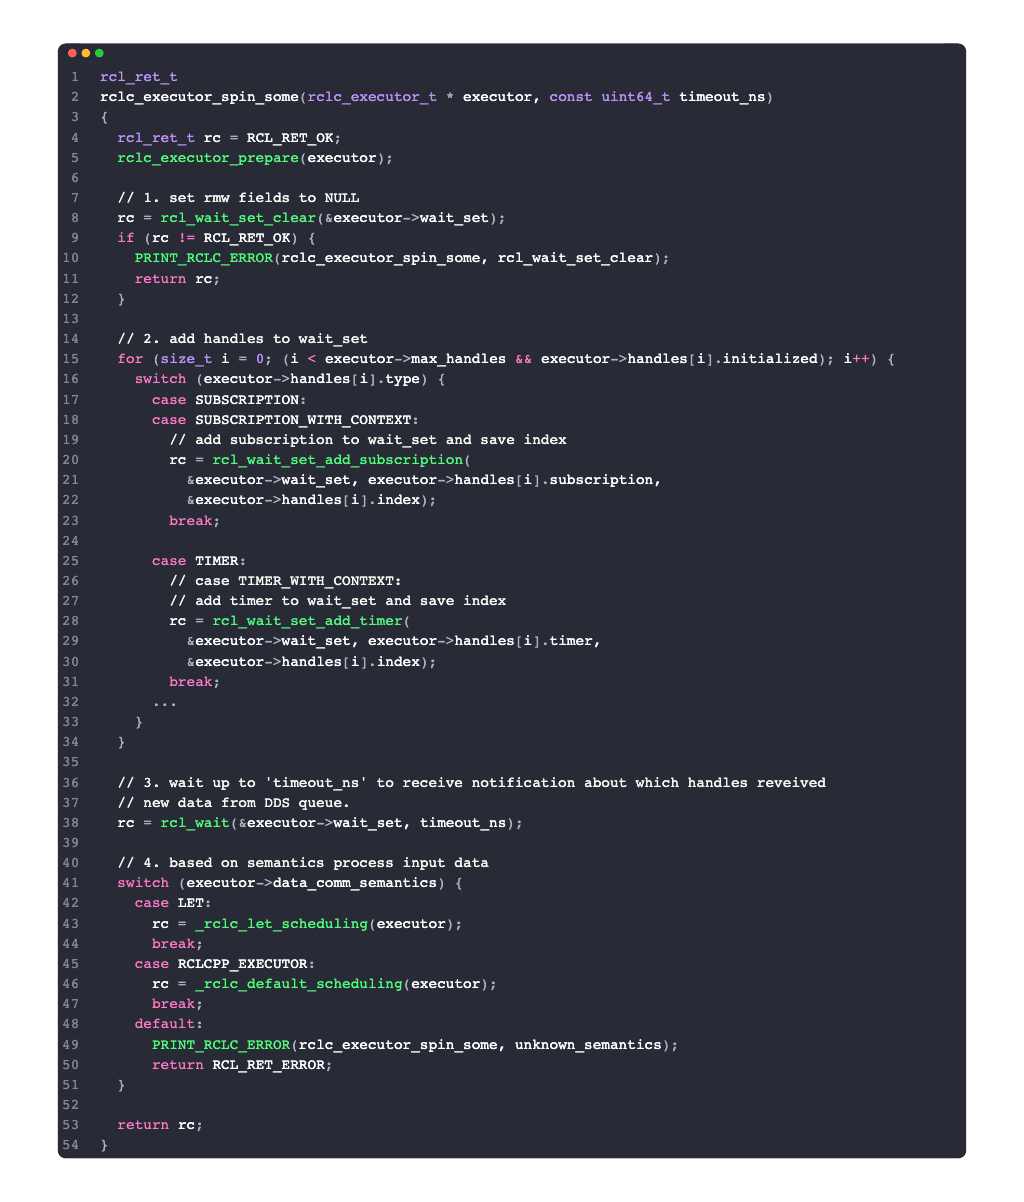
\includegraphics[width=1\linewidth]{Img/code/rclc/rclc_executor_spin_some.png}
    \caption{rclc\_executor\_spin\_some code}
    \vspace{-0.1in}
\end{figure}

\subsubsection{\api{rclc\_executor\_spin(rclc\_executor\_t * executor)}}
The function \api{rclc\_executor\_spin} calls \api{rclc\_executor\_spin\_some} indefinitely as long as the ROS system is alive. This might create a high performance load on your processor.

\subsubsection{\api{rclc\_executor\_spin\_period(rclc\_executor\_t * executor, const uint64\_t period)}}
The function \api{rclc\_executor\_spin\_period} calls \api{rclc\_executor\_spin\_some} periodically (as defined with the argument period) as long as the ROS system is alive.

\subsubsection{\apiarg{rclc\_executor\_spin\_one\_period}{rclc\_executor\_t * executor, const uint64\_t period}}
This is a function used by \api{rclc\_executor\_spin\_period} to spin one time. The purpose is to test the accuracy of the \api{spin\_period} function in the unit tests.

\subsection{Clean-Up Phase}
\subsubsection{\apiarg{rclc\_executor\_fini}{}}
The function \api{rlce\_executor\_fini} frees the dynamically allocated memory of the executor.

\subsection{RCL convenience functions}
The rclc package also provides a number of convenience functions, which make it easier to create the RCL-objects \textit{rcl\_node\_t}, \textit{rcl\_subscription\_t}, \textit{rcl\_timer\_t} and \textit{rcl\_publisher\_t}. Convenience functions:
\begin{itemize}
    \item \api{rclc\_support\_init()}
    \item \api{rclc\_support\_init\_with\_options()}
    \item \api{rclc\_support\_fini()}
    \item \api{rclc\_node\_init\_default()}
    \item \api{rclc\_publisher\_init\_default()}
    \item \api{rclc\_subscription\_init\_default()}
    \item \api{rclc\_timer\_init\_default()}
\end{itemize}

\subsection{Examples}
\subsubsection{Example of real-time embedded application use-case}
In embedded systems, real-time behavior is approached by using the time-triggered paradigm, which means that the processes are periodically activated. Processes can be assigned priorities to allow pre-emptions. Figure~\ref{fig:sch1} shows an example, in which three processes with fixed periods are shown. The middle and lower process are preempted multiple times depicted with empty dashed boxes. To each process one or multiple tasks can be assigned, as shown in Figure~\ref{fig:sch2}. These tasks are executed sequentially, which is often called cooperative scheduling.
\begin{figure*}[t!]
    \begin{minipage}[t]{0.5\textwidth}
        \setcaptionwidth{2in}
        %\hspace{0pt}
        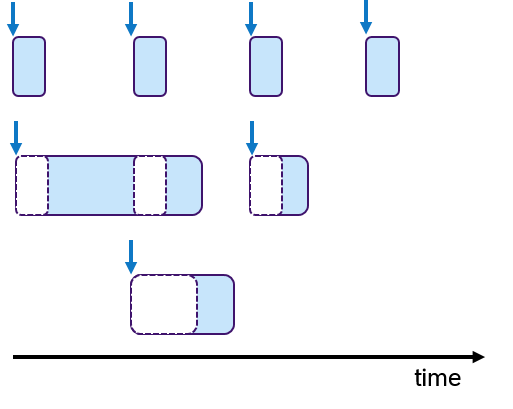
\includegraphics[scale = 0.8]{Img/scheduling_01.png}
        \caption{Fixed periodic preemptive scheduling}
        \label{fig:sch1} %\vspace{-10pt}
    \end{minipage}
    \begin{minipage}[t]{0.5\textwidth}
        \setcaptionwidth{2in}
        %\hspace{0pt}
        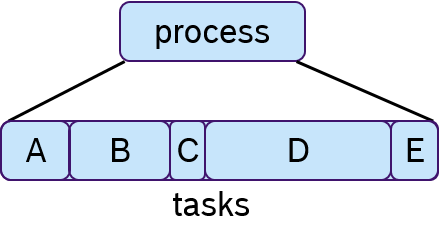
\includegraphics[scale = 0.8]{Img/scheduling_02.png}
        \caption{Processes with sequentially executed tasks}
        \label{fig:sch2} %\vspace{-10pt}
    \end{minipage}
\end{figure*}

With sequential execution the co-operative scheduling of tasks within a process can be modeled. The trigger condition is used to periodically activate the process which will then execute all callbacks in a pre-defined order. Data will be communicated using the LET-semantics. Every Executor is executed in its own tread, to which an appropriate priority can be assigned.

In the following example, the Executor is setup with 4 handles. We assume a process has three subscriptions \textit{sub1}, \textit{sub2}, \textit{sub3}. The sequential processing order is given by the order as they are added to the Executor. A timer \textit{timer} defines the period. The \textit{trigger\_one} with the parameter timer is used, so that whenever the timer is ready, all callbacks are processed. Finally the data communication semantics LET is defined.

\forget{
\begin{lstlisting}[language=python, caption=real-time embedded application use-case]
#include "rcl_executor/let_executor.h"

// define subscription callback
void my_sub_cb1(const void * msgin)
{
    // ...
}
// define subscription callback
void my_sub_cb2(const void * msgin)
{
    // ...
}
// define subscription callback
void my_sub_cb3(const void * msgin)
{
    // ...
}

// define timer callback
void my_timer_cb(rcl_timer_t * timer, int64_t last_call_time)
{
    // ...
}

// necessary ROS 2 objects
rcl_context_t context;
rcl_node_t node;
rcl_subscription_t sub1, sub2, sub3;
rcl_timer_t timer;
rcle_let_executor_t exe;

// define ROS context
context = rcl_get_zero_initialized_context();
// initialize ROS node
rcl_node_init(&node, &context,...);
// create subscriptions
rcl_subscription_init(&sub1, &node, ...);
rcl_subscription_init(&sub2, &node, ...);
rcl_subscription_init(&sub3, &node, ...);
// create a timer
rcl_timer_init(&timer, &my_timer_cb, ... );
// initialize executor with four handles
rclc_executor_init(&exe, &context, 4, ...);
// define static execution order of handles
rclc_executor_add_subscription(&exe, &sub1, &my_sub_cb1, ALWAYS);
rclc_executor_add_subscription(&exe, &sub2, &my_sub_cb2, ALWAYS);
rclc_executor_add_subscription(&exe, &sub3, &my_sub_cb3, ALWAYS);
rclc_executor_add_timer(&exe, &timer);
// trigger when handle 'timer' is ready
rclc_executor_set_trigger(&exe, rclc_executor_trigger_one, &timer);
// select LET-semantics
rclc_executor_data_comm_semantics(&exe, LET);
// spin forever
rclc_executor_spin(&exe);  
\end{lstlisting}}
\begin{figure}[htbp!]
    \centering
    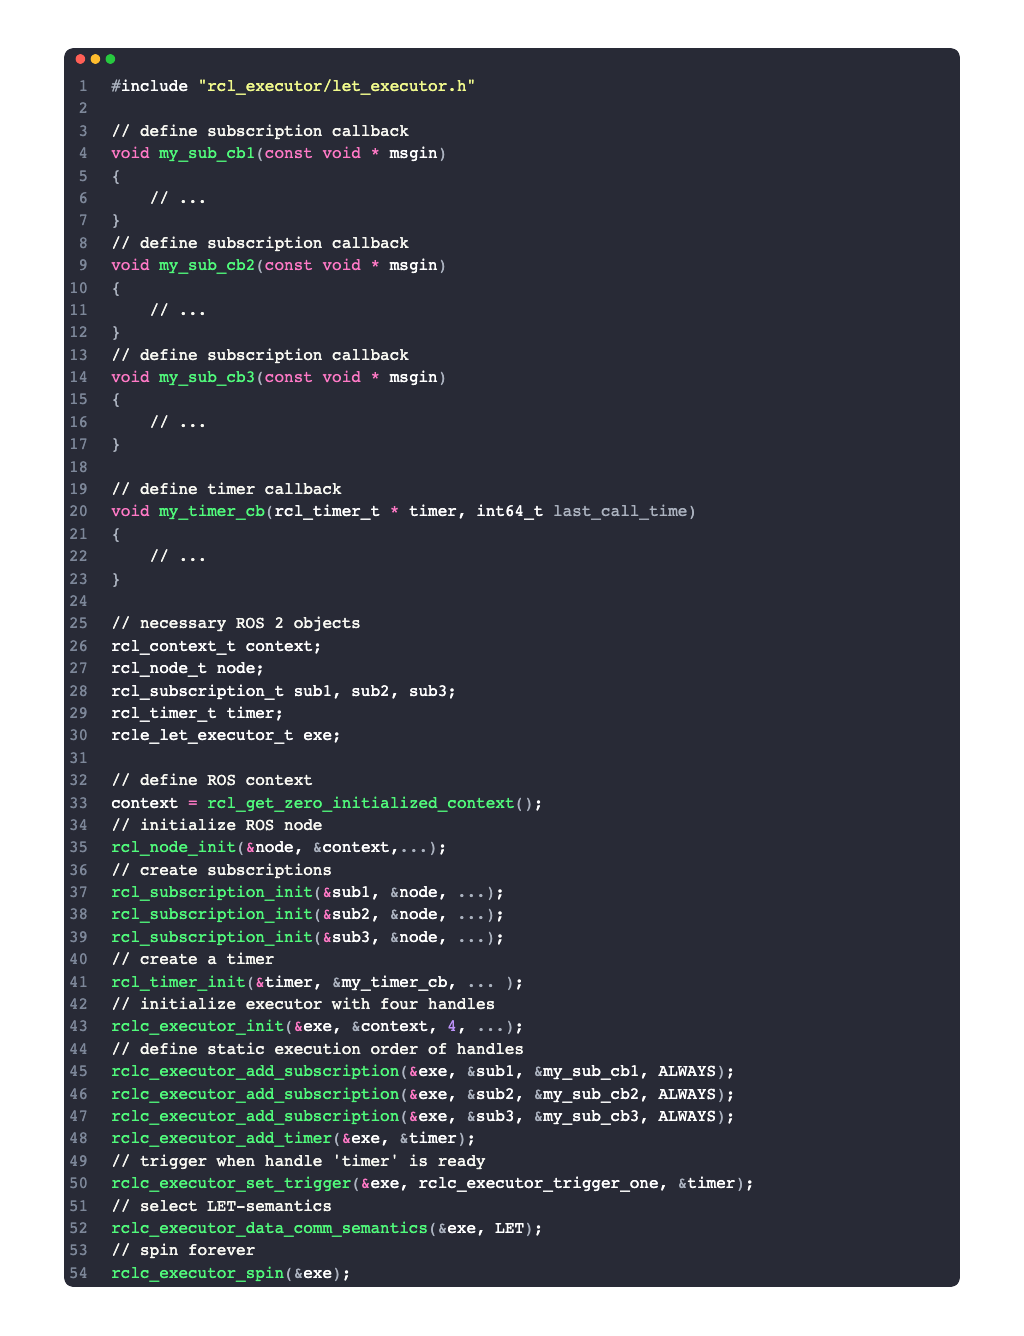
\includegraphics[width=1\linewidth]{Img/code/example1.png}
    \caption{real-time embedded application use-case}\label{f:example1}
    \vspace{-0.1in}
\end{figure}


\subsubsection{Example of sense-plan-act pipeline in mobile robotics}
A common design paradigm in mobile robotics is a control loop, consisting of several phases: A sensing phase to acquire sensor data, a plan phase for localization and path planning and an actuation-phase to steer the mobile robot. Of course, more phases are possible, here these three phases shall serve as an example. Such a processing pipeline is shown in Figure~\ref{f:sensePlanActScheme}. Typically multiple sensors are used to perceive the environment. For example an IMU and a laser scanner. The quality of localization algorithms highly depend on how old such sensor data is when it is processed. Ideally the latest data of all sensors should be processed. One way to achieve this is to execute first all sensor drivers in the sense-phase and then process all algorithms in the plan-phase.
\begin{figure}[htbp!]
    \centering
    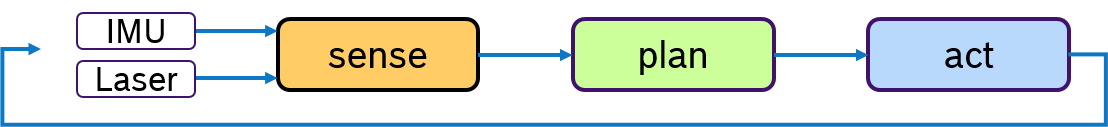
\includegraphics[width=0.75\linewidth]{Img/sensePlanActScheme.png}
    \caption{Multiple sensors driving a Sense-Plan-Act pipeline}\label{f:sensePlanActScheme}
    \vspace{-0.1in}
\end{figure}

In this example we want to realise a sense-plan-act pipeline in a single thread. The trigger condition is demonstrated by activating the sense-phase when both data for the Laser and IMU are available. Three executors are necessary \textit{exe\_sense}, \textit{exe\_plan} and \textit{exe\_act}. The two sensor acquisition callbacks \textit{sense\_Laser} and \textit{sense\_IMU} are registered in the Executor exe\_sense. The trigger condition \textit{ALL} is responsible to activate the sense-phase only when all data for these two callbacks are available. Finally all three Executors are spinning using a while-loop and the \api{spin\_some} function.
\forget{
\begin{lstlisting}[language=python, caption=real-time embedded application use-case]
...
rcl_subscription_t sense_Laser, sense_IMU, plan, act;
rcle_let_executor_t exe_sense, exe_plan, exe_act;
// initialize executors
rclc_executor_init(&exe_sense, &context, 2, ...);
rclc_executor_init(&exe_plan, &context, 1, ...);
rclc_executor_init(&exe_act, &context, 1, ...);
// executor for sense-phase
rclc_executor_add_subscription(&exe_sense, &sense_Laser, &my_sub_cb1, ON_NEW_DATA);
rclc_executor_add_subscription(&exe_sense, &sense_IMU, &my_sub_cb2, ON_NEW_DATA);
rclc_let_executor_set_trigger(&exe_sense, rclc_executor_trigger_all, NULL);
// executor for plan-phase
rclc_executor_add_subscription(&exe_plan, &plan, &my_sub_cb3, ON_NEW_DATA);
// executor for act-phase
rclc_executor_add_subscription(&exe_act, &act, &my_sub_cb4, ON_NEW_DATA);

// spin all executors
while (true) {
    rclc_executor_spin_some(&exe_sense);
    rclc_executor_spin_some(&exe_plan);
    rclc_executor_spin_some(&exe_act);
}
\end{lstlisting}}
\begin{figure}[htbp!]
    \centering
    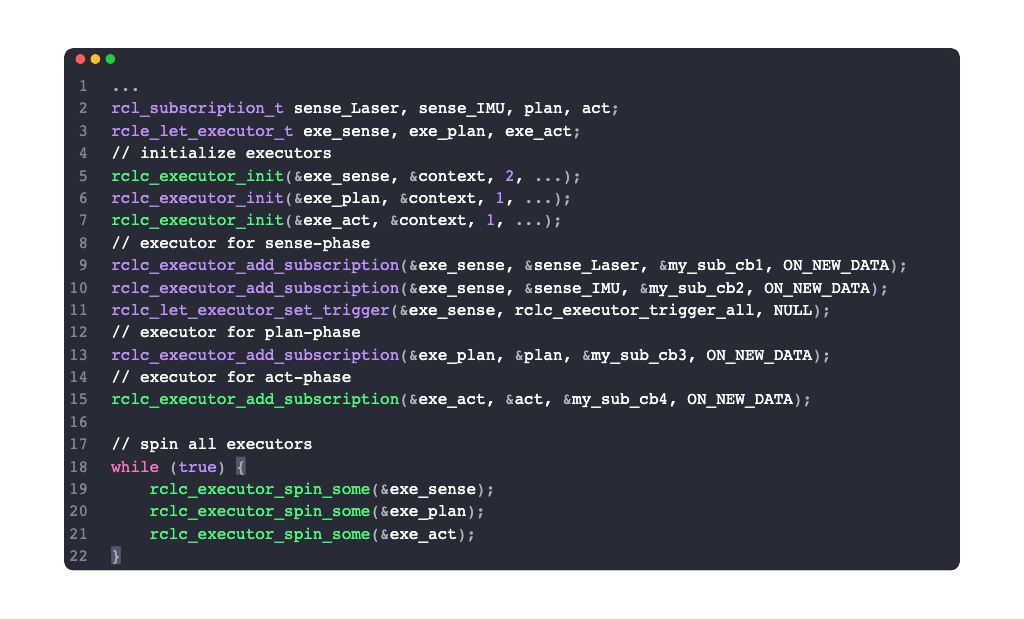
\includegraphics[width=1\linewidth]{Img/code/example2.png}
    \caption{sense-plan-act pipeline in mobile robotics}\label{f:example2}
    \vspace{-0.1in}
\end{figure}


\subsubsection{Example of synchronization of multiple rates}
Often multiple sensors are being used to sense the environment for mobile robotics. While an IMU sensor provides data samples at a very high rate (e.g. 500 Hz), laser scans are available at a much slower frequency (e.g. 10Hz) determined by the revolution time. Then the challenge is, how to deterministically fuse sensor data with different frequencies. This problem is depicted in Figure~\ref{f:sensorFusion_01}.
\begin{figure}[htb!]
    \centering
    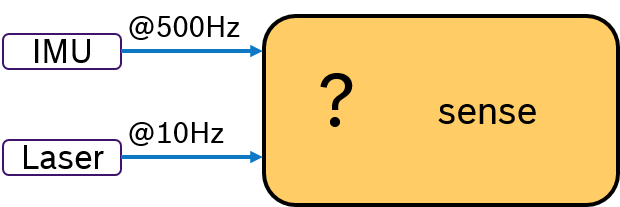
\includegraphics[width=0.75\linewidth]{Img/sensorFusion_01.png}
    \caption{How to deterministically process multi-frequent sensor data}\label{f:sensorFusion_01}
    \vspace{-0.1in}
\end{figure}

An Alternative would be to evaluate the IMU sample and the laser scan by synchronizing their frequency. For example by processing always 50 IMU samples with one laser scan. This approach is shown in Figure \ref{f:sensorFusion_02}. A pre-processing callback aggregates the IMU samples and sends an aggregated message with 50 samples at 10Hz rate. Now both messages have the same frequency. With a trigger condition, which fires when both messages are available, the sensor fusion algorithm can expect always synchronized input data.
\begin{figure}[htb!]
    \centering
    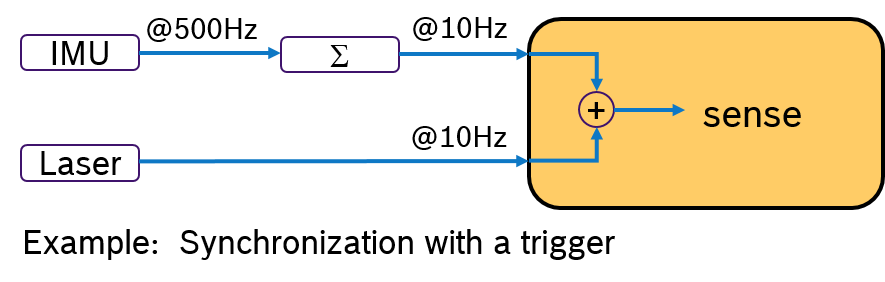
\includegraphics[width=0.75\linewidth]{Img/sensorFusion_02.png}
    \caption{How to deterministically process multi-frequent sensor data}\label{f:sensorFusion_02}
    \vspace{-0.1in}
\end{figure}

The sensor fusion synchronizing the multiple rates with a trigger is shown below.
\forget{
\begin{lstlisting}[language=python, caption=real-time embedded application use-case]
...
rcl_subscription_t aggr_IMU, sense_Laser, sense_IMU;
rcle_let_executor_t exe_aggr, exe_sense;
// initialize executors
rclc_executor_init(&exe_aggr, &context, 1, ...);
rclc_executor_init(&exe_sense, &context, 2, ...);
// executor for aggregate IMU data
rclc_executor_add_subscription(&exe_aggr, &aggr_IMU, &my_sub_cb1, ON_NEW_DATA);
// executor for sense-phase
rclc_executor_add_subscription(&exe_sense, &sense_Laser, &my_sub_cb2, ON_NEW_DATA);
rclc_executor_add_subscription(&exe_sense, &sense_IMU, &my_sub_cb3, ON_NEW_DATA);
rclc_executor_set_trigger(&exe_sense, rclc_executor_trigger_all, NULL);

// spin all executors
while (true) {
    rclc_executor_spin_some(&exe_aggr);
    rclc_executor_spin_some(&exe_sense);
}
\end{lstlisting}}
\begin{figure}[htbp!]
    \centering
    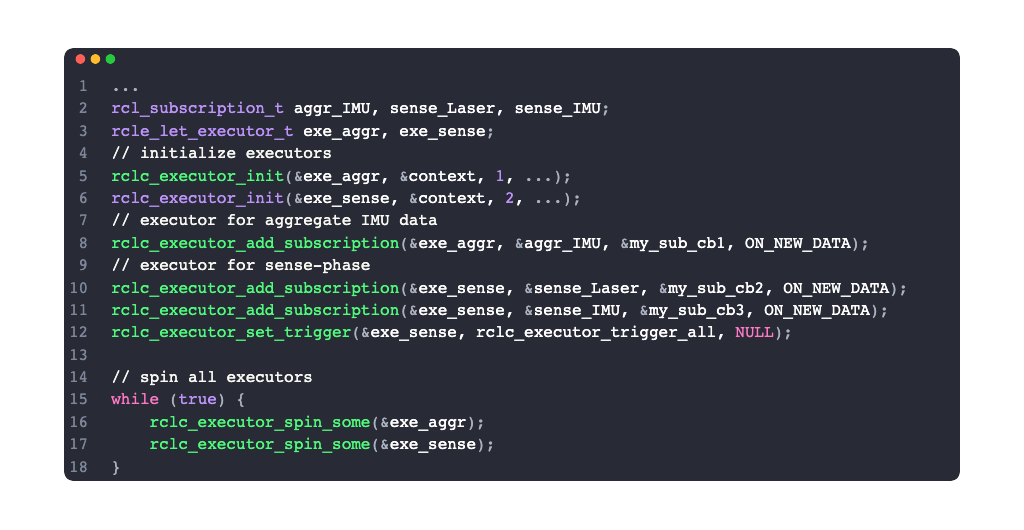
\includegraphics[width=1\linewidth]{Img/code/example3.png}
    \caption{synchronization of multiple rates}\label{f:example3}
    \vspace{-0.1in}
\end{figure}


Another idea would be to actively request for IMU data only when a laser scan is received. This concept is shown in Figure \ref{f:sensorFusion_03}. Upon arrival of a laser scan message, first, a message with aggregated IMU samples is requested. Then, the laser scan is processed and later the sensor fusion algorithm. An Executor, which would support sequential execution of callbacks, could realize this idea.
\begin{figure}[htb!]
    \centering
    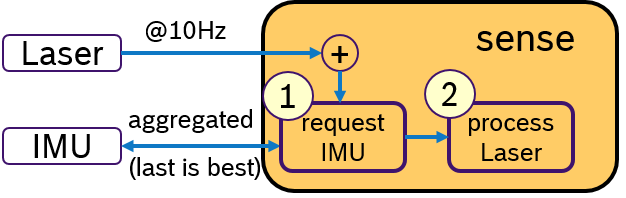
\includegraphics[width=0.75\linewidth]{Img/sensorFusion_03.png}
    \caption{Synchronization of multiple input data with a trigger}\label{f:sensorFusion_03}
    \vspace{-0.1in}
\end{figure}

The setup for the sensor fusion using sequential execution is shown below. Note, that the sequential order is sense\_IMU, which will request the aggregated IMU message, and then sense\_Laser while the trigger will fire, when a laser message is received.
\forget{
\begin{lstlisting}[language=python, caption=real-time embedded application use-case]
...
rcl_subscription_t sense_Laser, sense_IMU;
rcle_let_executor_t exe_sense;
// initialize executor
rclc_executor_init(&exe_sense, &context, 2, ...);
// executor for sense-phase
rclc_executor_add_subscription(&exe_sense, &sense_IMU, &my_sub_cb1, ALWAYS);
rclc_executor_add_subscription(&exe_sense, &sense_Laser, &my_sub_cb2, ON_NEW_DATA);
rclc_executor_set_trigger(&exe_sense, rclc_executor_trigger_one, &sense_Laser);
// spin
rclc_executor_spin(&exe_sense);
\end{lstlisting}}
\begin{figure}[htbp!]
    \centering
    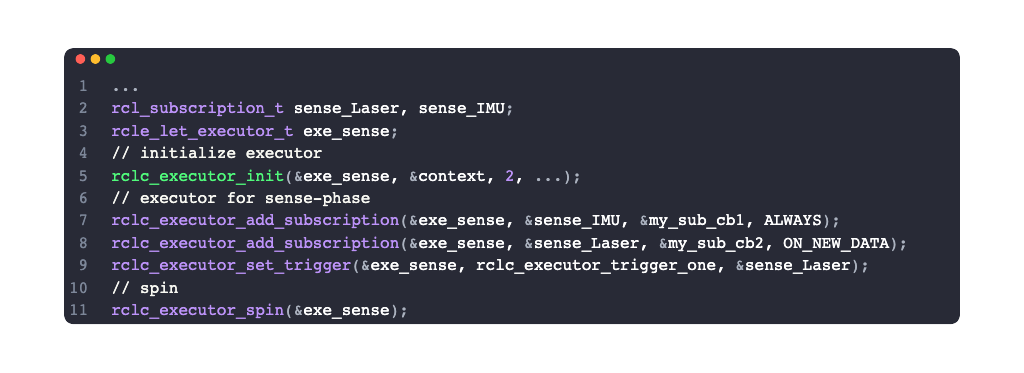
\includegraphics[width=1\linewidth]{Img/code/example32.png}
    \caption{synchronization of multiple rates}\label{f:example32}
    \vspace{-0.1in}
\end{figure}

\subsubsection{Example of high-priority processing path}
Often a robot has to fulfill several activities at the same time. For example following a path and avoiding obstacles. While path following is a permanent activity, obstacle avoidance is triggered by the environment and should be immediately reacted upon. Therefore one would like to specify priorities to activities. This is depicted in Figure \ref{f:highPriorityPath}. Assuming a simplified control loop with the activities sense-plan-act, the obstacle avoidance, which might temporarily stop the robot, should be processed before the planning phase. In this example we assume that these activities are processed in one thread.
\begin{figure}[htb!]
    \centering
    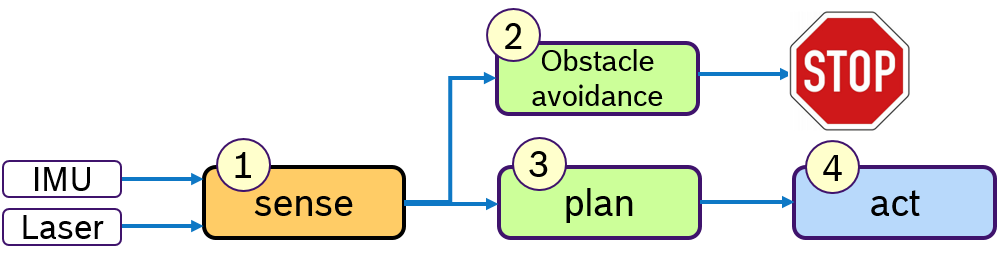
\includegraphics[width=0.75\linewidth]{Img/highPriorityPath.png}
    \caption{Managing high priority path with sequential order}\label{f:highPriorityPath}
    \vspace{-0.1in}
\end{figure}

This example shows the sequential processing order to execute the obstacle avoidance obst\_avoid after the callbacks of the sense-phase and before the callback of the planning phase plan. The control loop is started when a laser message is received. Then an aggregated IMU message is requested, like in the example above. Then all the other callbacks are always executed. This assumes that these callbacks communicate via a global data structure. Race conditions cannot occur, because the callbacks run all in one thread.
\forget{
\begin{lstlisting}[language=python, caption=real-time embedded application use-case]
...
rcl_subscription_t sense_Laser, sense_IMU, plan, act, obst_avoid;
rcle_let_executor_t exe;
// initialize executors
rclc_executor_init(&exe, &context, 5, ...);
// define processing order
rclc_executor_add_subscription(&exe, &sense_IMU, &my_sub_cb1, ALWAYS);
rclc_executor_add_subscription(&exe, &sense_Laser, &my_sub_cb2, ON_NEW_DATA);
rclc_executor_add_subscription(&exe, &obst_avoid, &my_sub_cb3, ALWAYS);
rclc_executor_add_subscription(&exe, &plan, &my_sub_cb4, ALWAYS);
rclc_executor_add_subscription(&exe, &act, &my_sub_cb5, ALWAYS);
rclc_executor_set_trigger(&exe, rclc_executor_trigger_one, &sense_Laser);
// spin
rclc_executor_spin(&exe);
\end{lstlisting}}
\begin{figure}[htbp!]
    \centering
    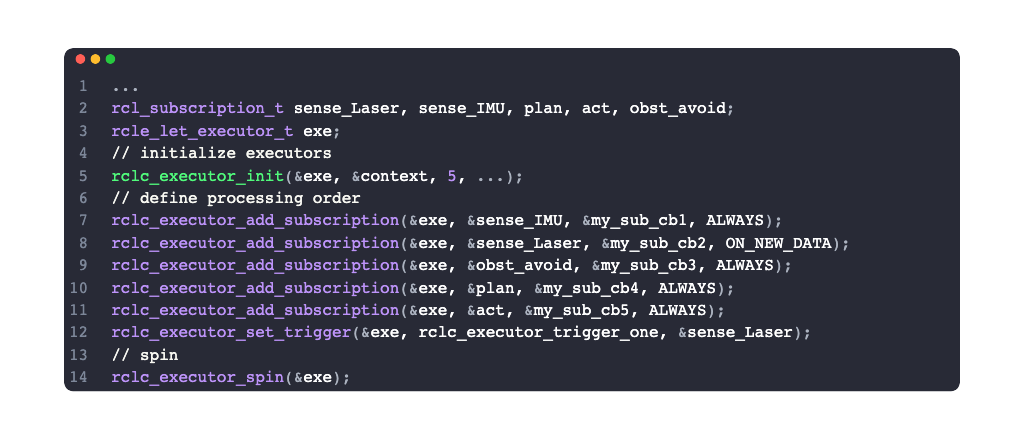
\includegraphics[width=1\linewidth]{Img/code/example4.png}
    \caption{high-priority processing path}\label{f:example4}
    \vspace{-0.1in}
\end{figure}

\subsection{Kernel Functions}
% - NOTE:===========================================================================
\subsubsection{\apiarg{\_rclc\_let\_scheduling}{rclc\_executor\_t * executor}}
\forget{
\begin{figure}[htbp!]
    \centering
    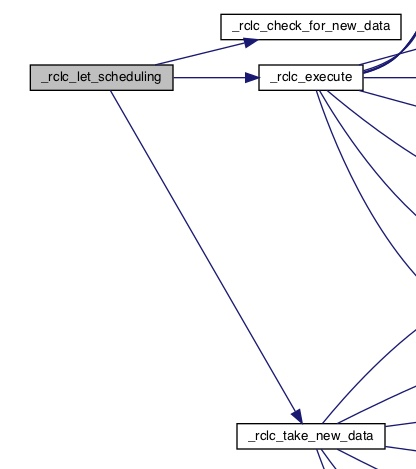
\includegraphics[width=0.3\linewidth]{Img/graph/rclc/let_scheduling_call.jpg}
    \caption{\_rclc\_let\_scheduling call}
    \vspace{-0.1in}
\end{figure}

\begin{figure}[htbp!]
    \centering
    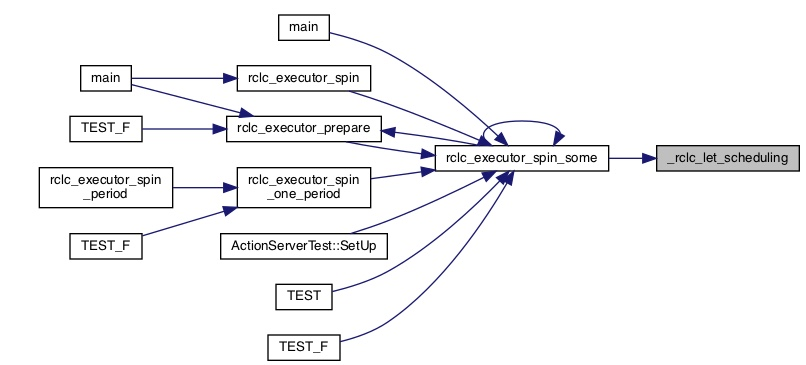
\includegraphics[width=1\linewidth]{Img/graph/rclc/let_scheduling_caller.jpg}
    \caption{\_rclc\_let\_scheduling caller}
    \vspace{-0.1in}
\end{figure}}

\begin{figure}[htbp!]
    \centering
    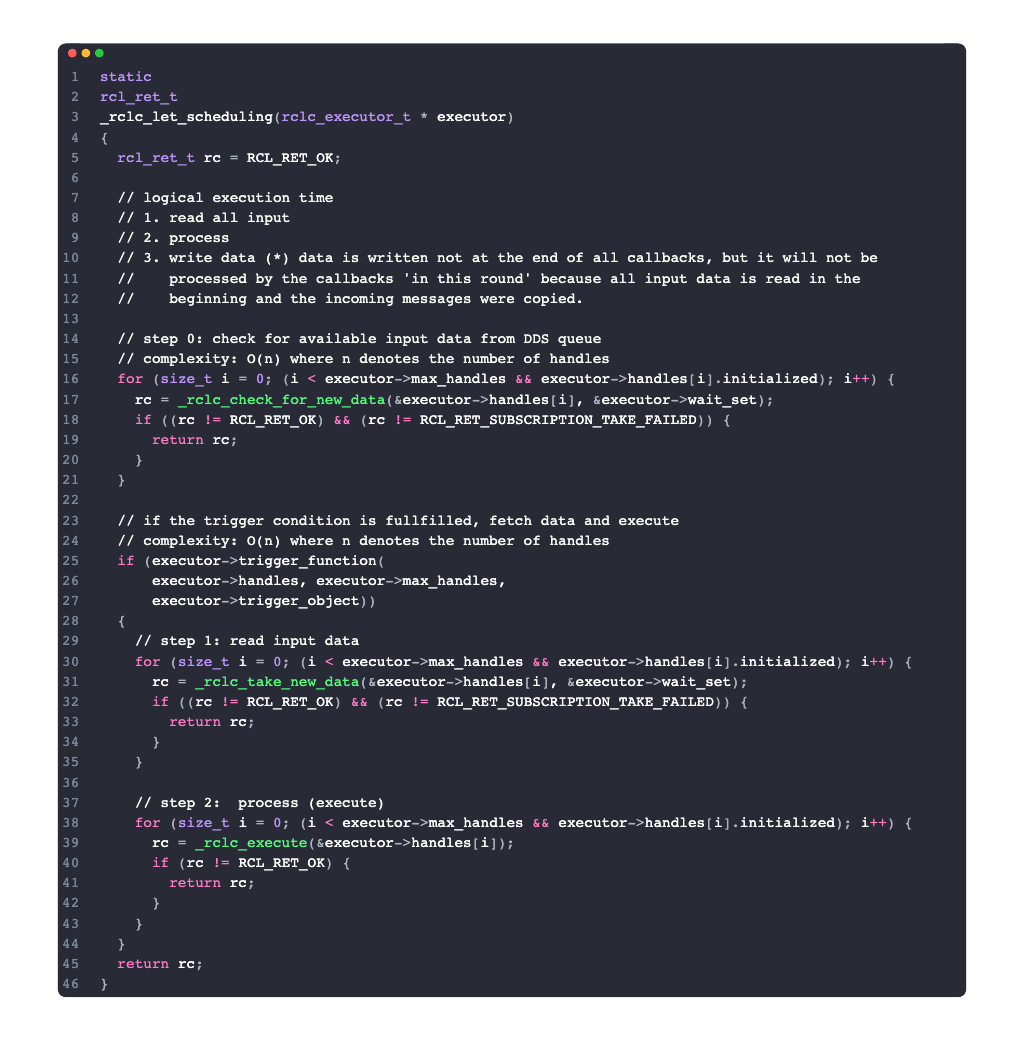
\includegraphics[width=1\linewidth]{Img/code/rclc/_rclc_let_scheduling.png}
    \caption{\_rclc\_let\_scheduling code}
    \vspace{-0.1in}
\end{figure}

% - NOTE:===========================================================================
\subsubsection{\apiarg{\_rclc\_default\_scheduling}{rclc\_executor\_t * executor}}
\begin{figure}[htbp!]
    \centering
    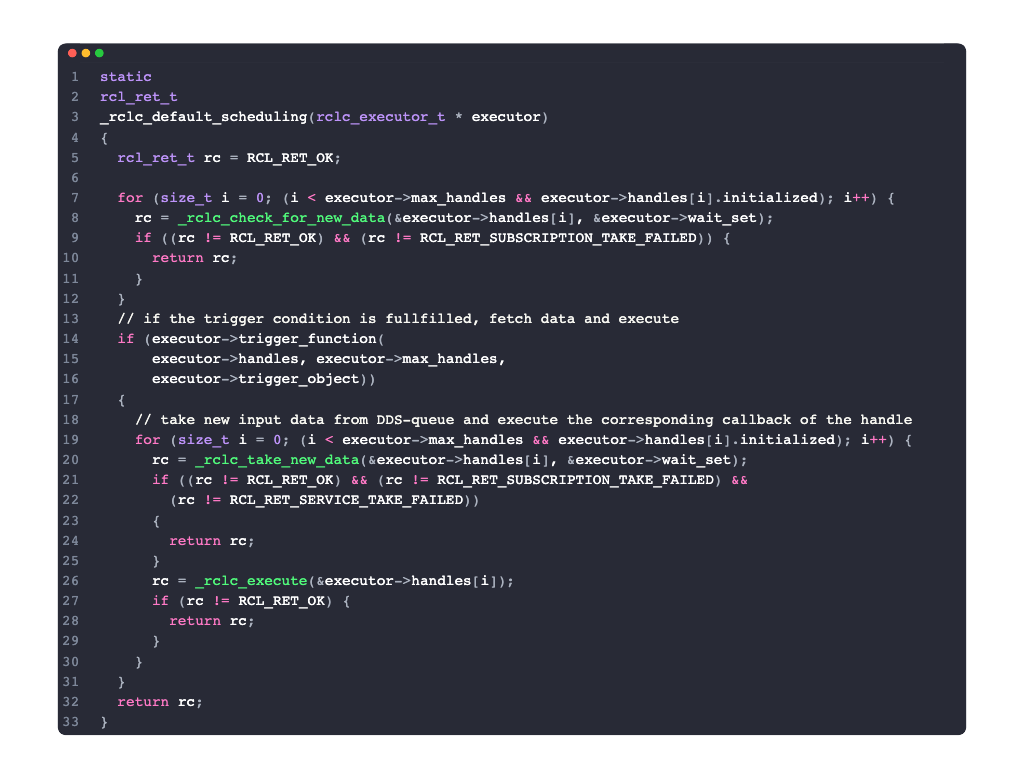
\includegraphics[width=1\linewidth]{Img/code/rclc/_rclc_default_scheduling.png}
    \caption{\_rclc\_let\_scheduling code}
    \vspace{-0.1in}
\end{figure}

% - NOTE:===========================================================================
\subsubsection{\apiarg{\_rclc\_check\_for\_new\_data}{rclc\_executor\_handle\_t * handle, rcl\_wait\_set\_t * wait\_set}}
\begin{figure}[htbp!]
    \centering
    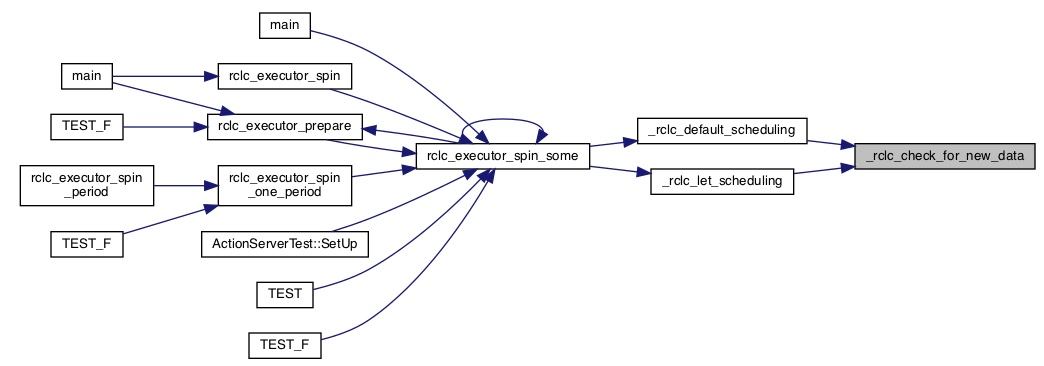
\includegraphics[width=1\linewidth]{Img/graph/rclc/check_for_new_data_caller.jpg}
    \caption{\_rclc\_let\_scheduling caller}
    \vspace{-0.1in}
\end{figure}

\begin{figure}[htbp!]
    \centering
    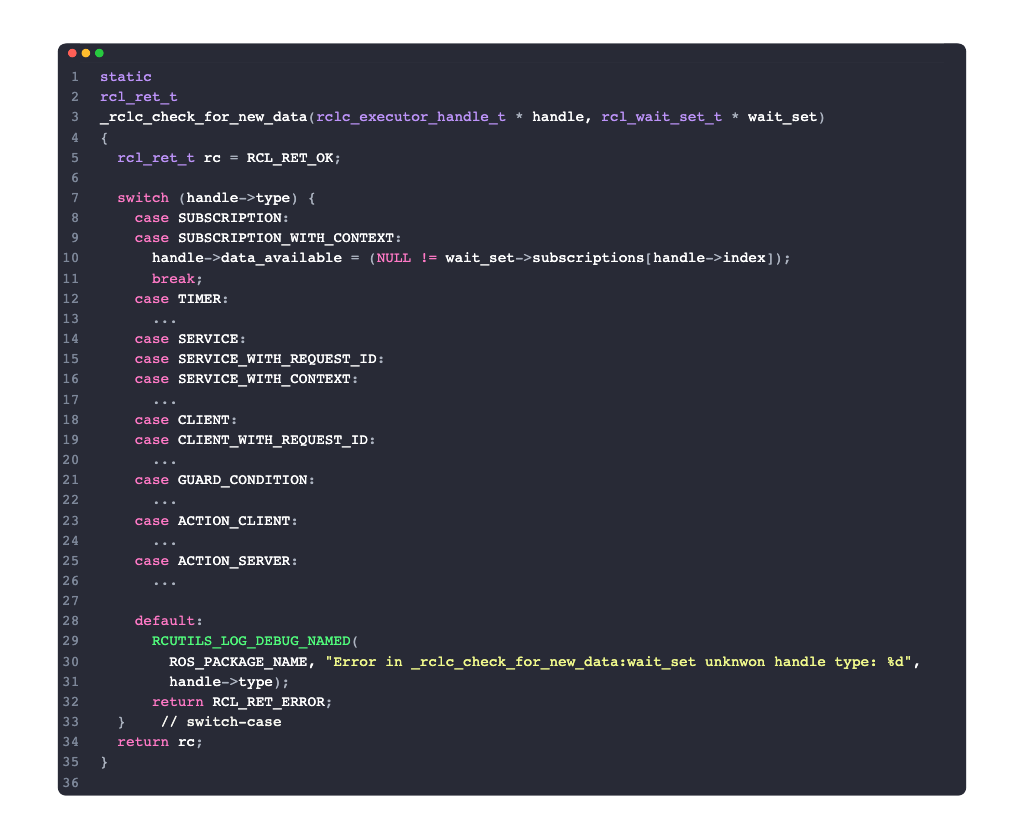
\includegraphics[width=1\linewidth]{Img/code/rclc/_rclc_check_for_new_data.png}
    \caption{\_rclc\_let\_scheduling code}
    \vspace{-0.1in}
\end{figure}

% - NOTE:===========================================================================
\subsubsection{\apiarg{\_rclc\_take\_new\_data}{rclc\_executor\_handle\_t * handle, rcl\_wait\_set\_t * wait\_set}}
\begin{figure}[htbp!]
    \centering
    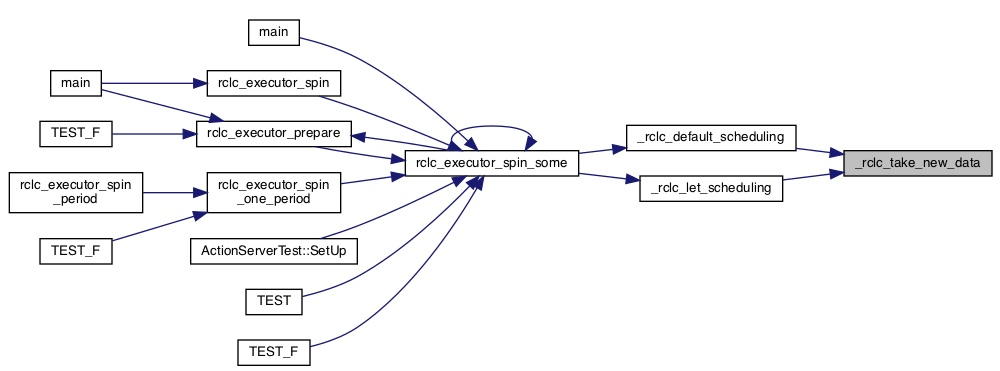
\includegraphics[width=1\linewidth]{Img/graph/rclc/take_new_data_caller.jpg}
    \caption{\_rclc\_let\_scheduling caller}
    \vspace{-0.1in}
\end{figure}

\begin{figure}[htbp!]
    \centering
    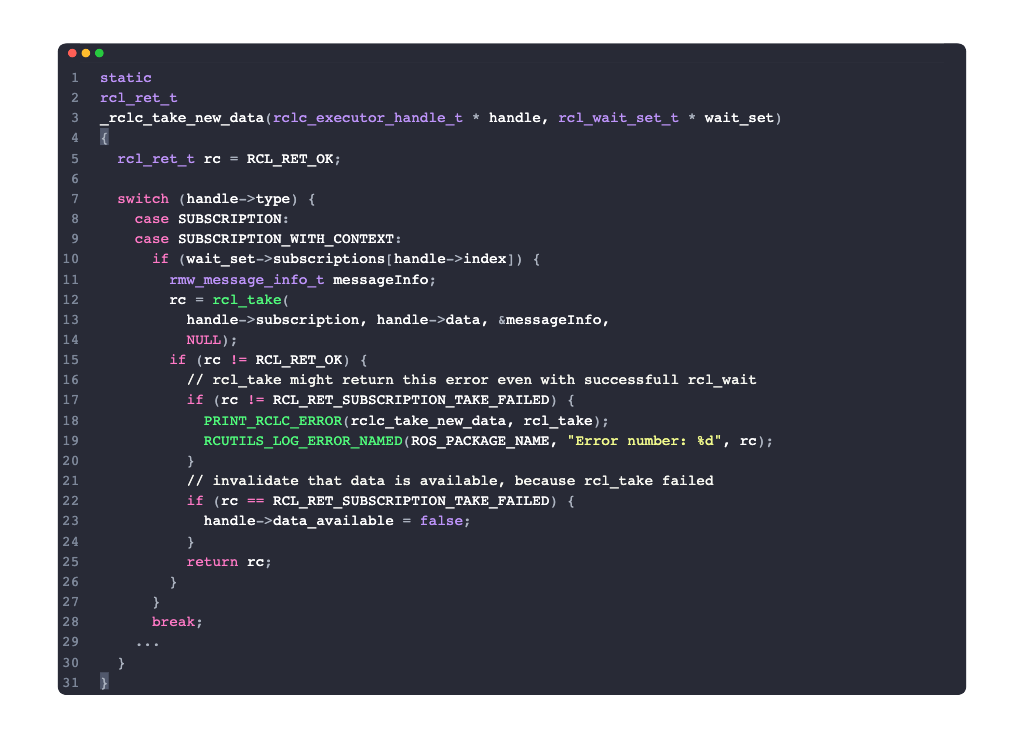
\includegraphics[width=1\linewidth]{Img/code/rclc/_rclc_tak_new_data.png}
    \caption{\_rclc\_let\_scheduling code}
    \vspace{-0.1in}
\end{figure}

% - NOTE:===========================================================================
\subsubsection{\apiarg{\_rclc\_execute}{rclc\_executor\_handle\_t * handle}}
\begin{figure}[htbp!]
    \centering
    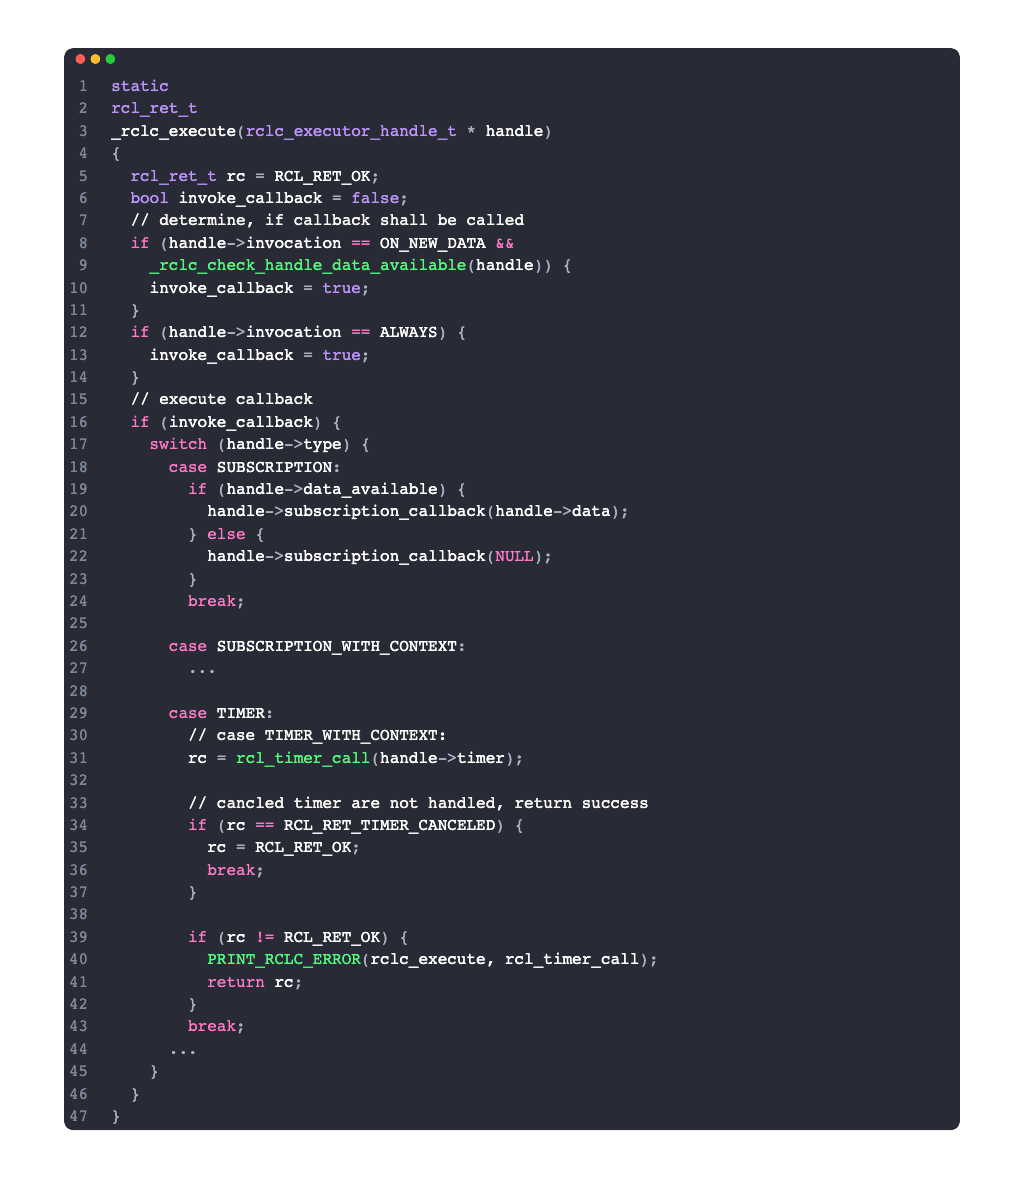
\includegraphics[width=1\linewidth]{Img/code/rclc/_rclc_execute.png}
    \caption{\_rclc\_execute code}
    \vspace{-0.1in}
\end{figure}

\section{RCL}
\subsection{RCL Layer Structures}
% - NOTE: -------------------------------------------------------------
\subsubsection{WORKING: wait.h}
\textbf{1. \str{rcl\_wait\_set\_t}}: 
\begin{figure}[htbp!]
    \centering
    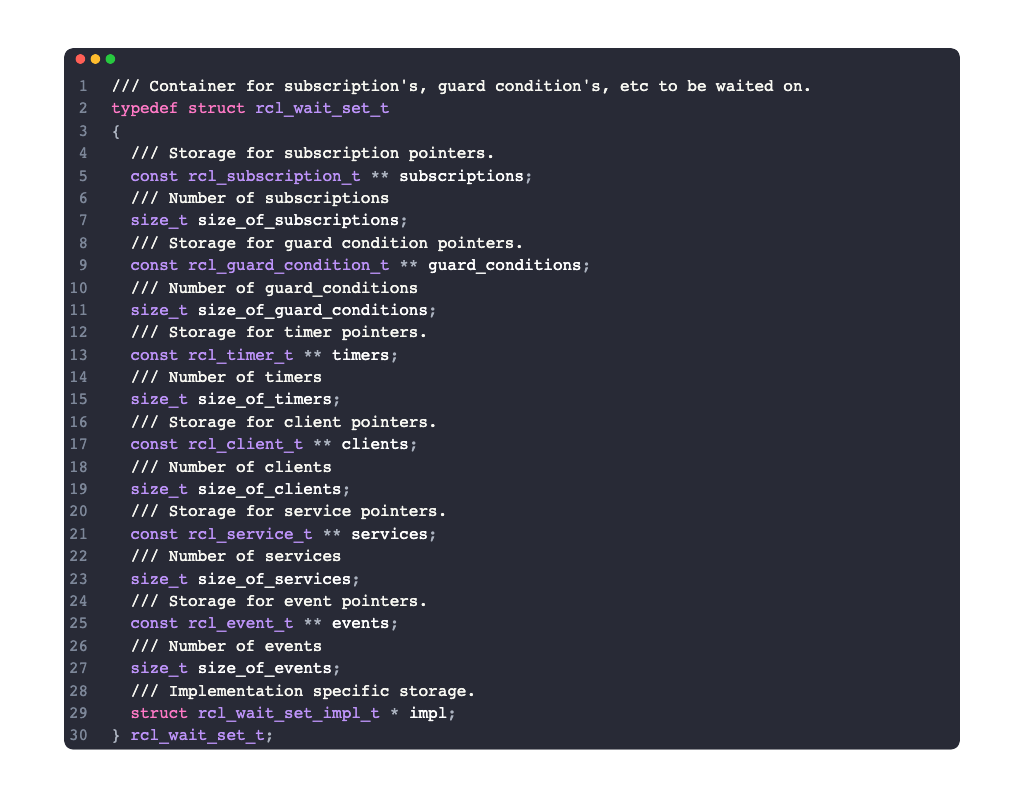
\includegraphics[width=1\linewidth]{Sec/Implementation/rcl/fig/rcl_wait_set_t.png}
    \caption{Structure: rcl\_wait\_set\_t}
    \vspace{-0.1in}
\end{figure}

\textbf{2. \str{rcl\_wait\_set\_impl\_t}}: 
\begin{figure}[htbp!]
    \centering
    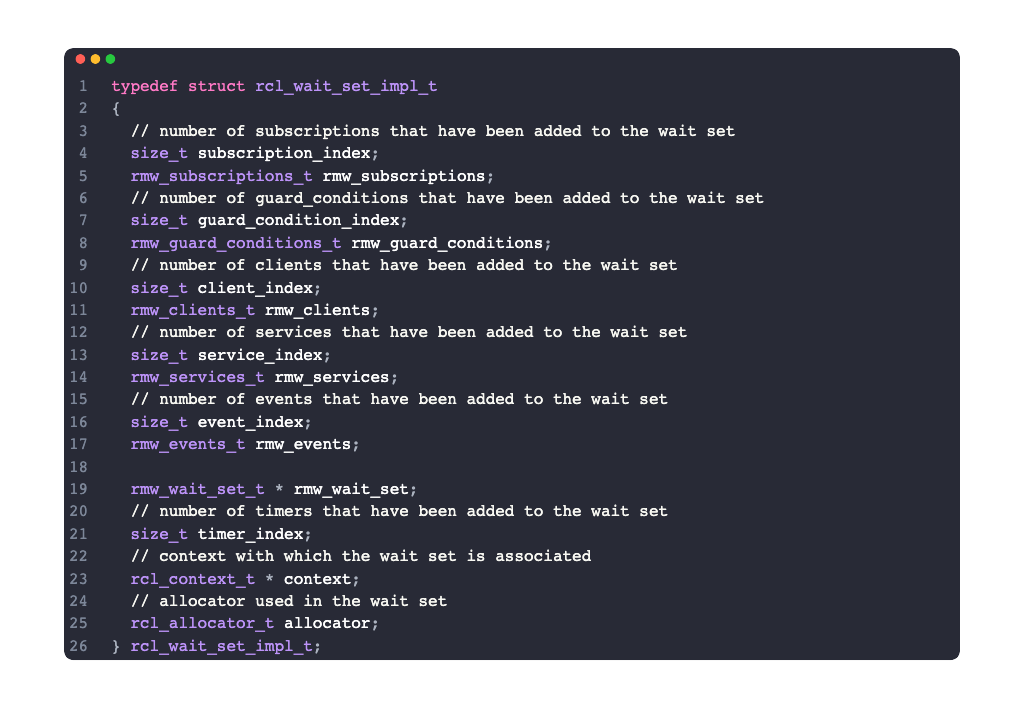
\includegraphics[width=1\linewidth]{Sec/Implementation/rcl/fig/rcl_wait_set_impl_t.png}
    \caption{Structure: rcl\_wait\_set\_impl\_t}
    \vspace{-0.1in}
\end{figure}
\subsection{RCL Layer APIs}
% - NOTE: -------------------------------------------------------------
\subsubsection{WORKING: wait.h}
Wait sets for waiting on messages/service requests and responses/timers to be ready.

\textbf{1. \apiarg{rcl\_wait\_set\_init}{rcl\_wait\_set\_t * wait\_set,
size\_t number\_of\_subscriptions,
size\_t number\_of\_guard\_conditions,
size\_t number\_of\_timers,
size\_t number\_of\_clients,
size\_t number\_of\_services,
size\_t number\_of\_events,
rcl\_context\_t * context,
rcl\_allocator\_t allocator}}: Initialize a rcl wait set with space for items to be waited on. This function allocates space for the subscriptions and other wait-able entities that can be stored in the wait set. It also sets the allocator to the given allocator and initializes the pruned member to be false. The \texttt{wait\_set struct} should be allocated and initialized to \texttt{NULL}. If the \texttt{wait\_set} is allocated but the memory is uninitialized the behavior is undefined. Calling this function on a wait set that has already been initialized will result in an error. A wait set can be reinitialized if \api{rcl\_wait\_set\_fini~()} was called on it.

\textbf{2. \apiarg{rcl\_wait\_set\_add\_subscription}{  rcl\_wait\_set\_t * wait\_set,
const rcl\_subscription\_t * subscription,
size\_t * index}}: Store a pointer to the given subscription in the next empty spot in the set. This function does not guarantee that the subscription is not already in the wait set. Also add the rmw representation to the underlying rmw array and increment the rmw array count.

\textbf{3. \apiarg{rcl\_wait}{rcl\_wait\_set\_t * wait\_set, int64\_t timeout}}: Block until the wait set is ready or until the timeout has been exceeded. This function will collect the items in the \str{rcl\_wait\_set\_t} and pass them to the underlying \api{rmw\_wait~()} function. The items in the wait set will be either left untouched or set to \str{NULL} after this function returns. Items that are not NULL are ready, where ready means different things based on the type of the item. For subscriptions this means there may be messages that can be taken, or perhaps that the state of the subscriptions has changed, in which case \api{rcl\_take~()} may succeed but return with taken == false. For guard conditions this means the guard condition was triggered.








% - NOTE: -------------------------------------------------------------
\subsubsection{WORKING: graph.h}
% - NOTE: -------------------------------------------------------------
\subsubsection{WORKING: init.h}
% - NOTE: -------------------------------------------------------------
\subsubsection{WORKING: guard\_condition.h}
\input{Sec/Implementation/rcl/rcl_static.tex}

\section{RMW}
\subsection{RMW Layer Structures}
% - NOTE: -------------------------------------------------------------
\subsubsection{WORKING: wait}
\textbf{1. \str{rmw\_wait\_set\_t}}: Container for guard conditions to be waited on.
\begin{figure}[htbp!]
    \centering
    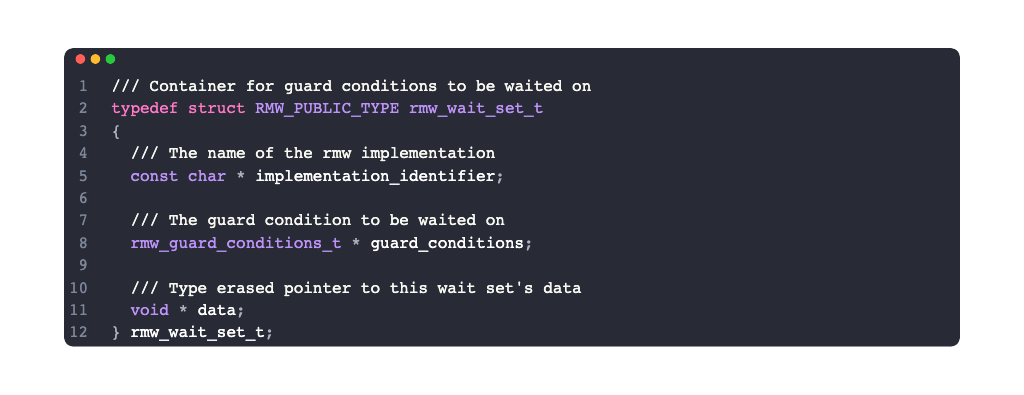
\includegraphics[width=1\linewidth]{Sec/Implementation/rmw/fig/rmw_wait_set_t.png}
    \caption{Structure: rmw\_wait\_set\_t}
    \vspace{-0.1in}
\end{figure}

\textbf{2. \str{rmw\_guard\_conditions\_t}}: Array of guard condition handles. An array of void * pointers representing type-erased middleware-specific guard conditions. The number of non-null entries may be smaller than the allocated size of the array. The number of guard conditions represented may be smaller than the allocated size of the array. The creator of this structure is responsible for allocating and de-allocating the array.
\begin{figure}[htbp!]
    \centering
    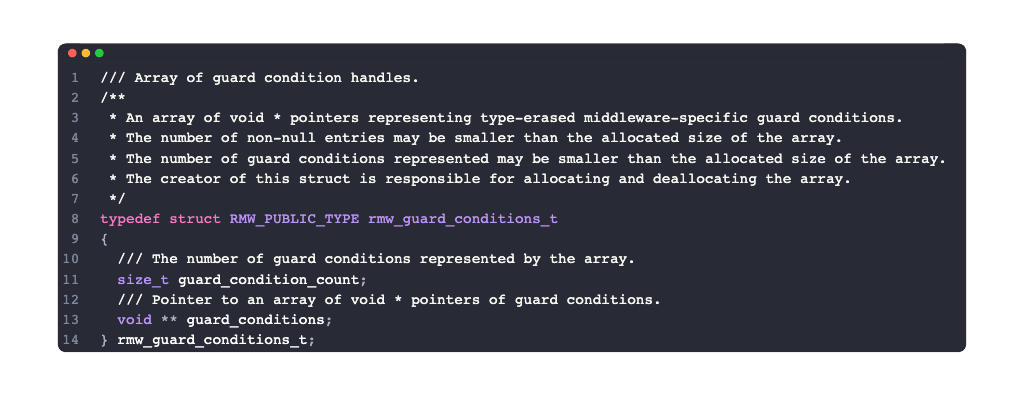
\includegraphics[width=1\linewidth]{Sec/Implementation/rmw/fig/rmw_guard_conditions_t.png}
    \caption{Structure: rmw\_guard\_conditions\_t}
    \vspace{-0.1in}
\end{figure}
\subsection{RMW Layer APIs}
% - NOTE: -------------------------------------------------------------
\subsubsection{INIT: rmw\_init.c}
\todo{HERE!!!!!}


% - NOTE: -------------------------------------------------------------
\subsubsection{WORKING: wait.h}

\textbf{1. \apiarg{rmw\_wait}{  rmw\_subscriptions\_t * subscriptions,
rmw\_guard\_conditions\_t * guard\_conditions,
rmw\_services\_t * services,
rmw\_clients\_t * clients,
rmw\_events\_t * events,
rmw\_wait\_set\_t * wait\_set,
const rmw\_time\_t * wait\_timeout}}: Waits on sets of different entities and returns when one is ready. This function adds middleware-specific conditions to the wait set and waits until one or more become ready, or until the timeout is reached. \footnote{Elapsed time is measured against the system clock. Timeout granularity is thus bound to that of the aforementioned clock and, depending on the underlying implementation, to that of platform-specific APIs to sleep and/or wait. \textbf{The amount of time this function actually waits may be either above or below the specified timeout.}} Called API \api{uxr\_run\_session\_until\_data~()} in XRCE-DDS layer.
\begin{figure}[htbp!]
    \centering
    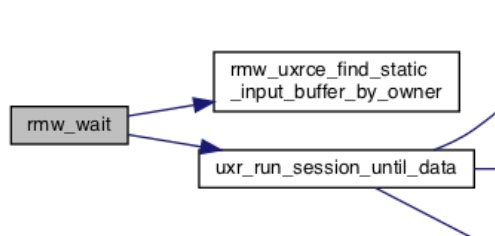
\includegraphics[width=0.5\linewidth]{Sec/Implementation/rmw/fig/rmw_wait().jpg}
    \caption{Function code: rmw\_wait()}
    \vspace{-0.1in}
\end{figure}
\input{Sec/Implementation/rmw/rmw_static.tex}

\section{XRCE-DDS}
\subsection{XRCE-DDS Layer Structures}
% - NOTE: -------------------------------------------------------------
\subsubsection{session.h}
\textbf{1. \str{uxrSession}}: 
\begin{figure}[htbp!]
    \centering
    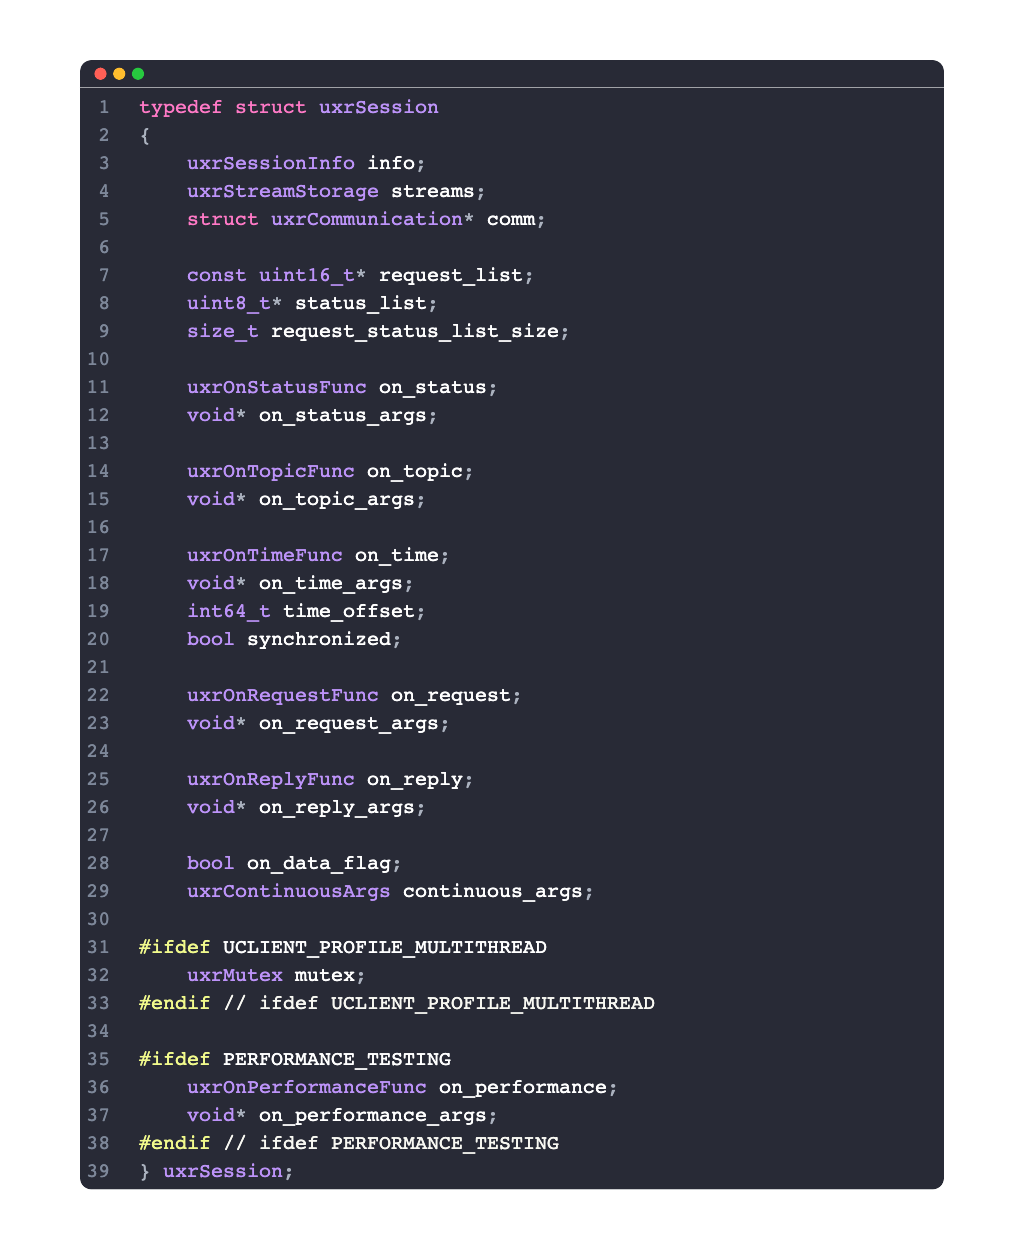
\includegraphics[width=1\linewidth]{Sec/Implementation/uxr/fig/uxrSession.png}
    \caption{Structure: uxrSession}
    \vspace{-0.1in}
\end{figure}


\subsection{XRCE-DDS Layer APIs}
% - NOTE: -------------------------------------------------------------
\subsubsection{session.c}

\textbf{1. \apiarg{uxr\_run\_session\_until\_data}{uxrSession* session, int timeout\_ms}}: Keeps communication between the Client and the Agent. This function involves the following actions:
\begin{itemize}
    \item [(1)] flushing all the output streams sending the data through the transport (e.g., UCP, UART\dots). This actions will be performed in a loop until a data message is received or the \str{timeout} is exceeded.
    \item [(2)] listening messages from the Agent calling the associated callback (topic, status, request and replies).
\end{itemize}

\begin{figure}[htbp!]
    \centering
    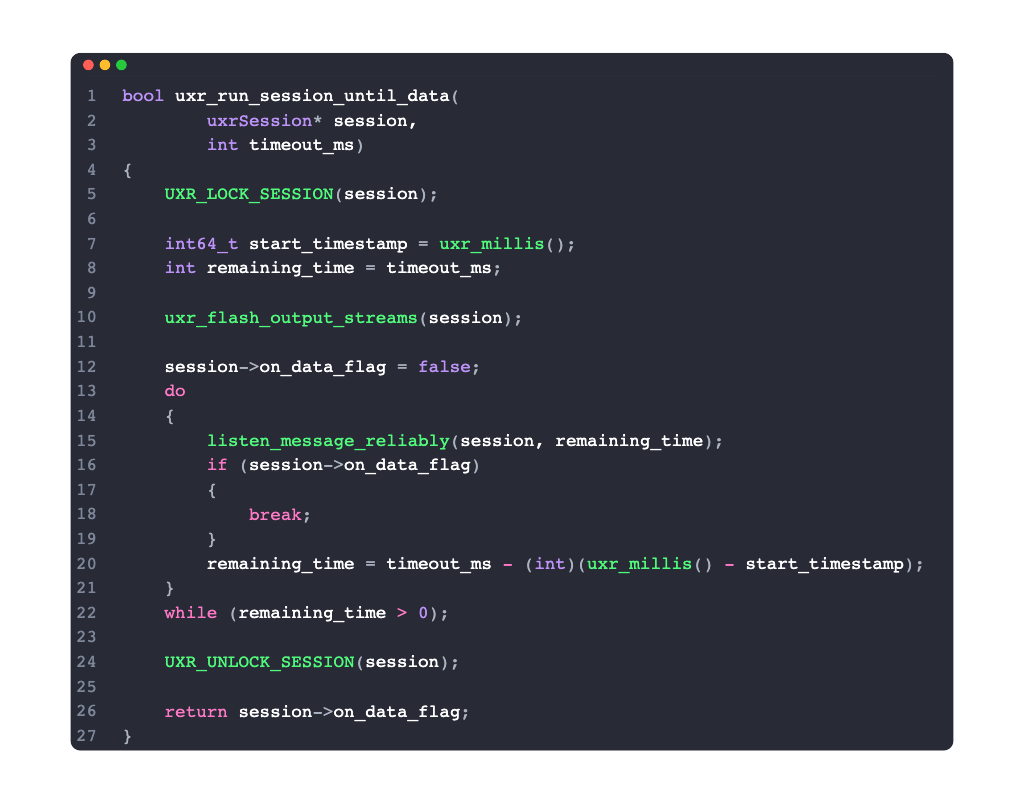
\includegraphics[width=1\linewidth]{Sec/Implementation/uxr/fig/uxr_run_session_until_data.png}
    \caption{Function code: uxr\_run\_session\_until\_data()}
    \vspace{-0.1in}
\end{figure}

As can be seen in function \api{uxr\_run\_session\_until\_data~()}, it first calls \apiarg{UXR\_LOCK\_SESSION}{session}, which finally invokes \apiarg{xSemaphoreTakeRecursive}{mutex->impl, portMAX\_DELAY} on FreeRTOS, or \apiarg{pthread\_mutex\_lock}{\&mutex->impl} on POSIX platform.

\textbf{2. \apiarg{uxr\_stream\_id}{uxrSession* session, int timeout\_ms}}:
\todo{HERE!!!!!!!!!!!!!!!!!!}

\textbf{3. \apiarg{uxr\_prepare\_best\_effort\_buffer\_to\_send}{uxrSession* session, int timeout\_ms}}:

\textbf{4. \apiarg{uxr\_stamp\_session\_header}{uxrSession* session, int timeout\_ms}}:
\input{Sec/Implementation/uxr/uxr_static.tex}

\section{USED POSIX API}
